\documentclass{beamer}

\setbeamertemplate{caption}[numbered]
\setbeamertemplate{footline}[frame number]
\beamertemplatenavigationsymbolsempty%

\usepackage[french]{babel}
\usepackage{fontspec}
\usepackage{graphicx}
\usepackage{hyperref}
\usepackage{luacode}
\usepackage{listings}

\begin{document}

% matos et fonctionnement
% ce qu'on a fait en tp 1A
% démo, exemples

  \begin{frame}{Nexys 2}{Mémoire}
    \begin{itemize}
      \item 16 Mo de RAM
      \item 16 Mo de flash
      \item 300 ko de BRAM
    \end{itemize}
    Actuellement 512 mots de 32 bits (en VHDL)
  \end{frame}

  \begin{frame}{Nexys 2}{Entrées sorties}
    Actuellement:
    \begin{itemize}
      \item 8 switchs
      \item 4 afficheurs 7 segments
      \item 8 Leds
    \end{itemize}
  \end{frame}

  \begin{frame}{Nexys 2}{Entrées sorties}
    \begin{itemize}
      \item RS-232
      \item VGA
    \end{itemize}
    mais:
    \begin{itemize}
      \item pas de contrôleur
      \item pas de gestion des adresses
    \end{itemize}
  \end{frame}

  \begin{frame}
    \centering
    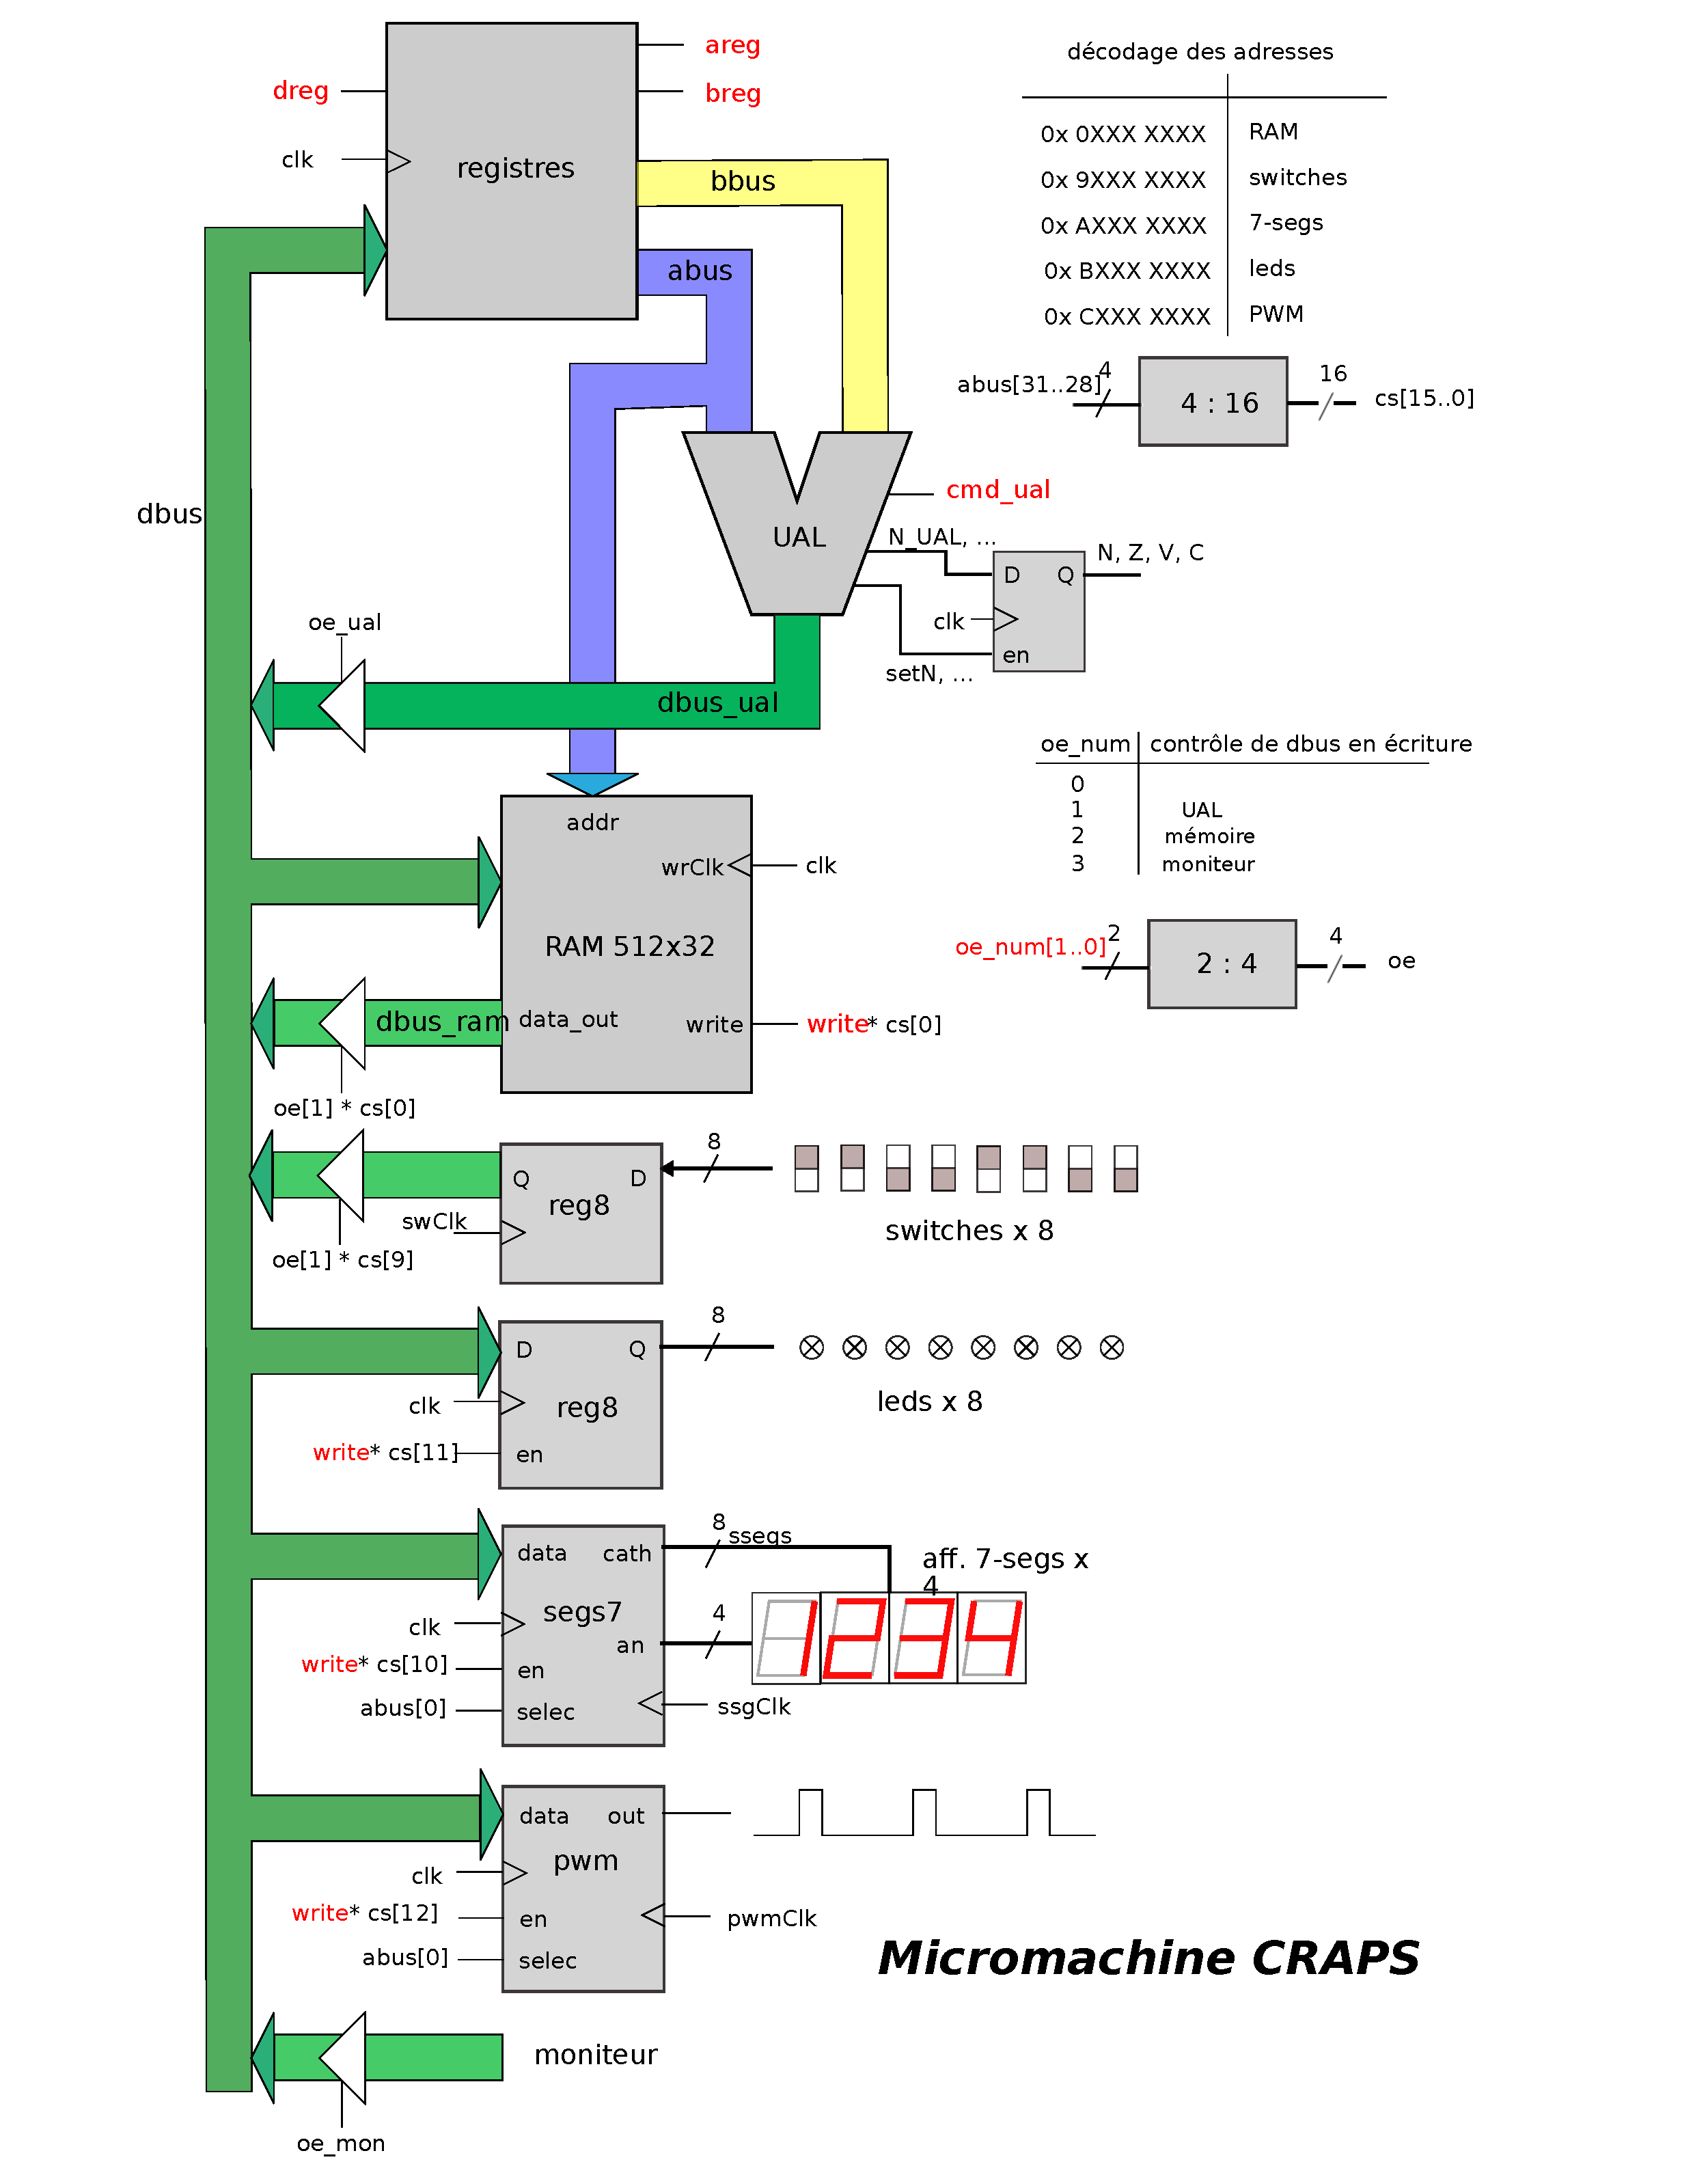
\includegraphics[height=\textheight, width=\textwidth, keepaspectratio]
                    {micromachine_fig.pdf}
  \end{frame}

  \begin{frame}{Registres}
    Jusqu'à 32 registres, pas tous implémentés
  \end{frame}

  \begin{frame}
    \centering
    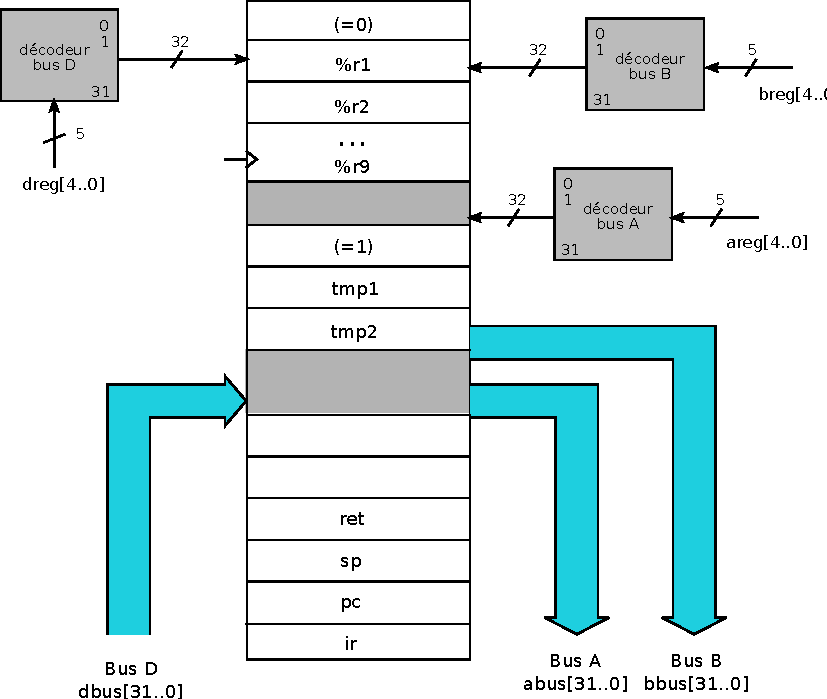
\includegraphics[height=\textheight, width=\textwidth, keepaspectratio]
                    {registres_fig.pdf}
  \end{frame}

  \begin{frame}{Compilation C}
    \begin{itemize}
      \item Récupérer le projet de TDL (backend x86 existant) et l'adapter
    \end{itemize}
  \end{frame}

  \begin{frame}{Interruptions}
    \begin{itemize}
      \item Ininterruptible
      \item Pas de test and set
    \end{itemize}
  \end{frame}

\end{document}

